\documentclass[Visionprosjekt.tex]{subfiles} 
\NormalTopp
\begin{document} 
  
%%%%%%%%%%%%%%%%%%%%%%%%%%%%%%%%%%%%%%%%%%%%%%%%
\section{Systembeskrivelse}
\label{sec:systembeskrivelse}
%%%%%%%%%%%%%%%%%%%%%%%%%%%%%%%%%%%%%%%%%%%%%%%%

Dette kapitlet vil gi en overordnet beskrivelse av prosjektoppgaven.
%1\textendash 2 
Prosjektet baserer seg på oppgaveteksten, se \refv{ved:oppgavetekst}. Prosjektgruppen har gjort en del endringer i forhold til oppgaveteksten, for å tilpasse systemet til vision-kameraet og de ulike sensorene som var tilgjengelige. Endringene går i hovedsak ut på plassering og nummerering av sensorer.  Anleggstegningen på 
\reff{fig:systemfigur2} viser oppbygningen av  transportbåndsystemet.


\begin{figure}[ht]
	\centering
		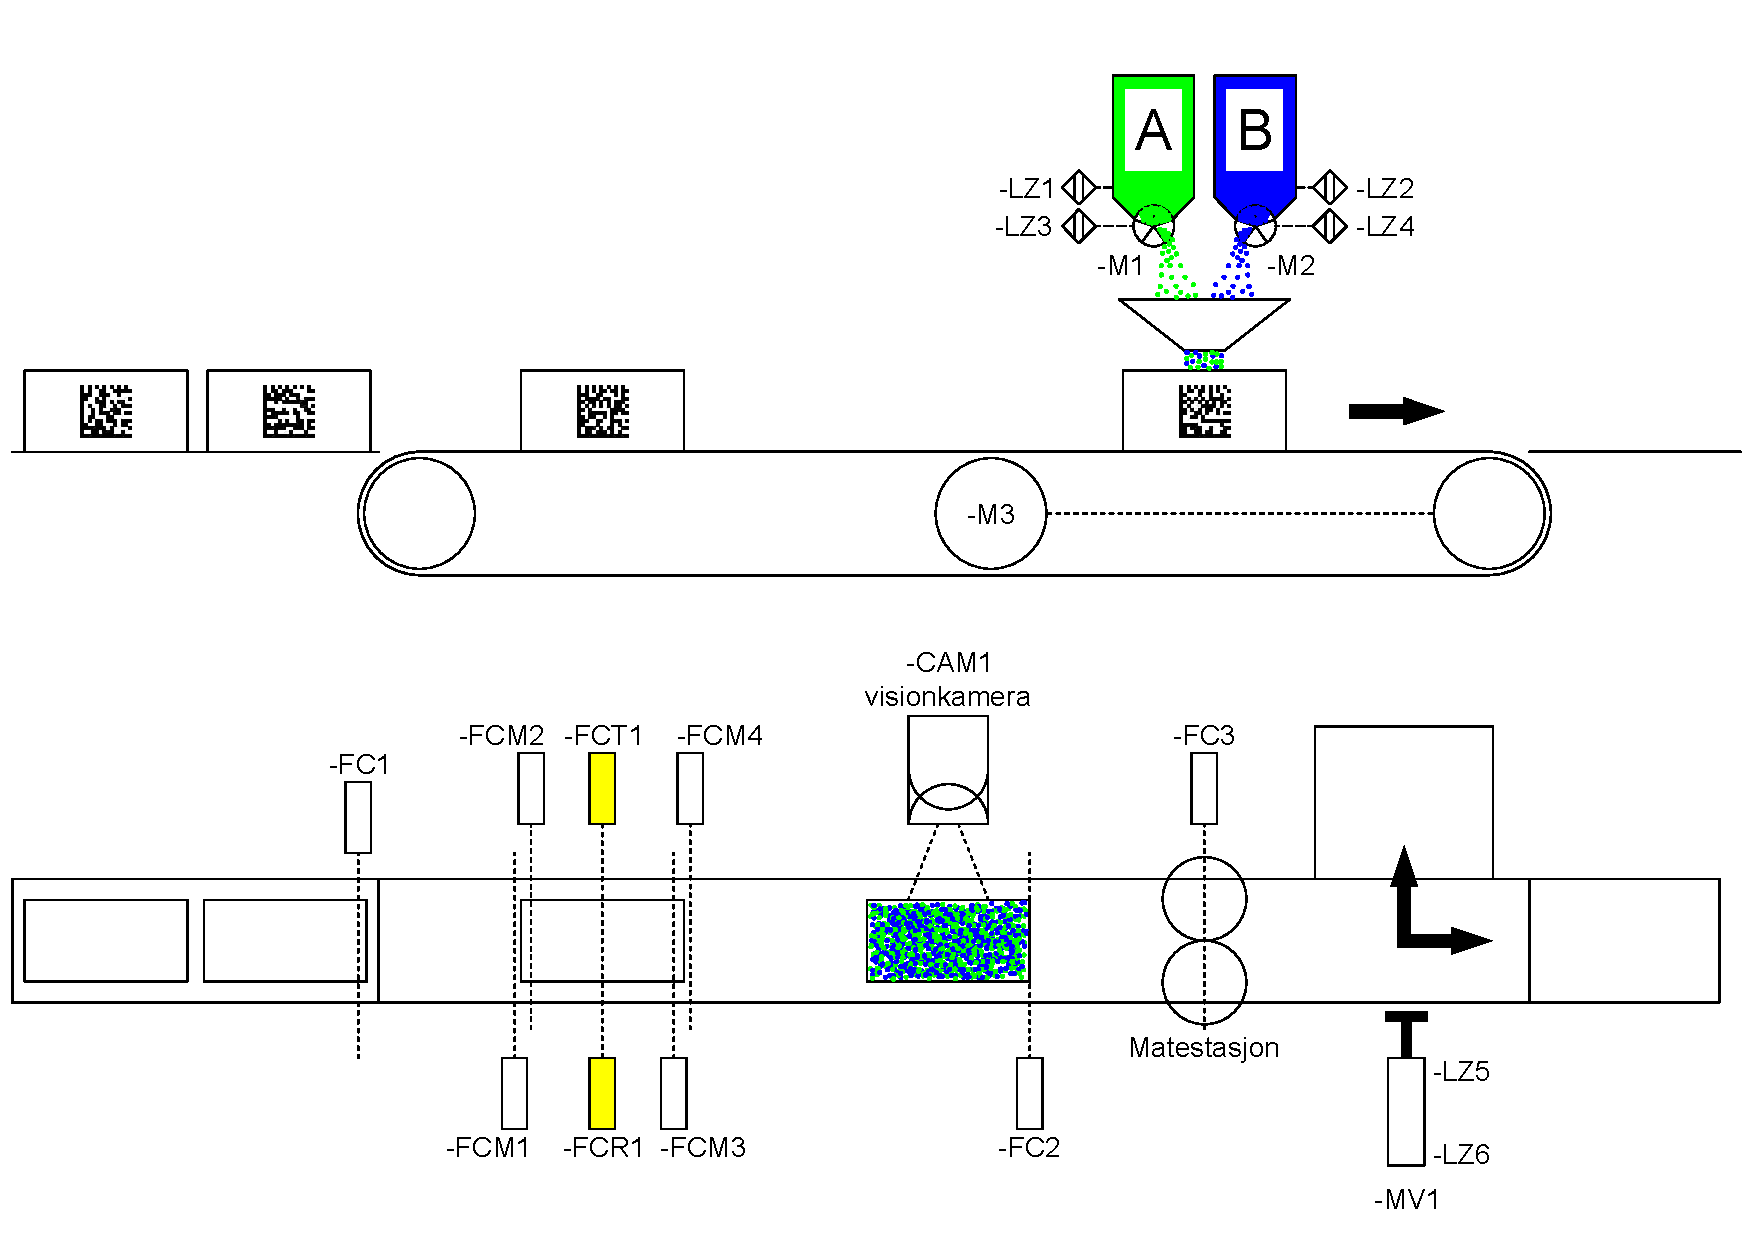
\includegraphics[width=\textwidth]{bilder/system2.pdf}
	\caption{Anleggstegning}
	\label{fig:systemfigur2}
\end{figure}


%
%\begin{figure}[ht]
	%\centering
		%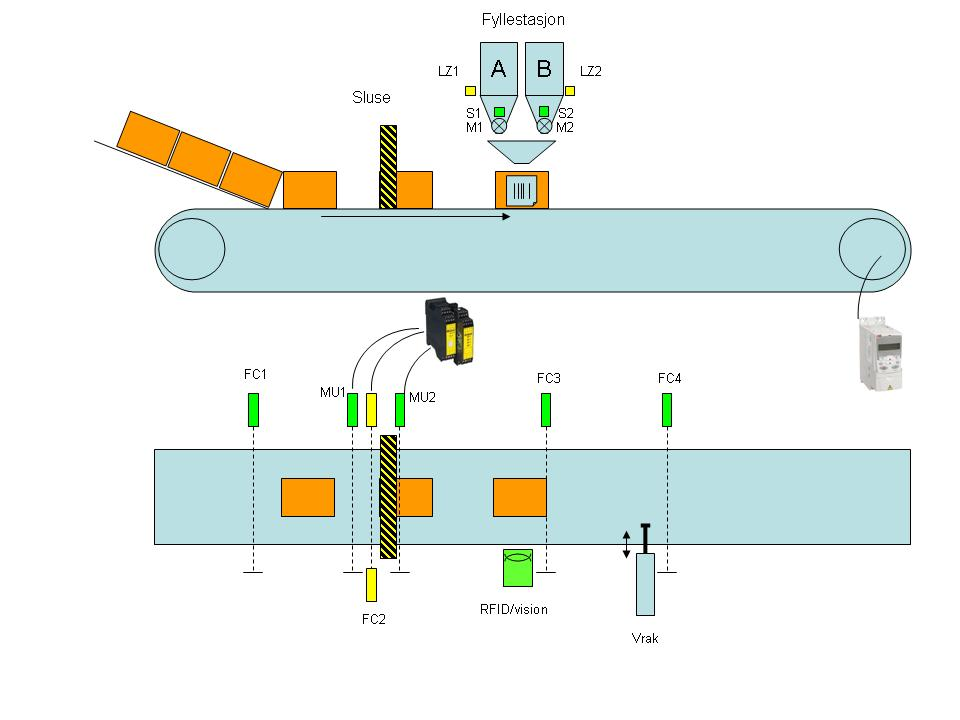
\includegraphics[width=\textwidth]{bilder/systemfigur.jpg}
	%\caption{Anleggstegning fra oppgaveteksten}
	%\label{fig:systemfigur}
%\end{figure}


Anlegget er koblet opp på et brett, hvor de ulike komponentene er plassert i henhold til \reff{fig:Arrangementstegning}. Forklaring til komponentreferansene i figuren finnes i \reft{tab:elliste}.


Et brukergrensesnitt er laget ved hjelp av WinCC. Her kan operatøren sette parametre, overvåke prosessen og logge alarmer og hendelser, i tillegg til å  styre anlegget manuelt  eller sette det i automatisk modus. 


%Systemet er styrt av en sekvens som kjører på en PLS, manuell kjøring er også mulig. %, og går fra et trinn til det, eller de neste ved å oppflylle gitte krav. 
Den automatiske modusen og sikkerhetssystemene som er benyttet i forbindelse med anlegget,  vil bli nærmere beskrevet i de neste underkapitlene.


\begin{figure}[ht]
	\centering
		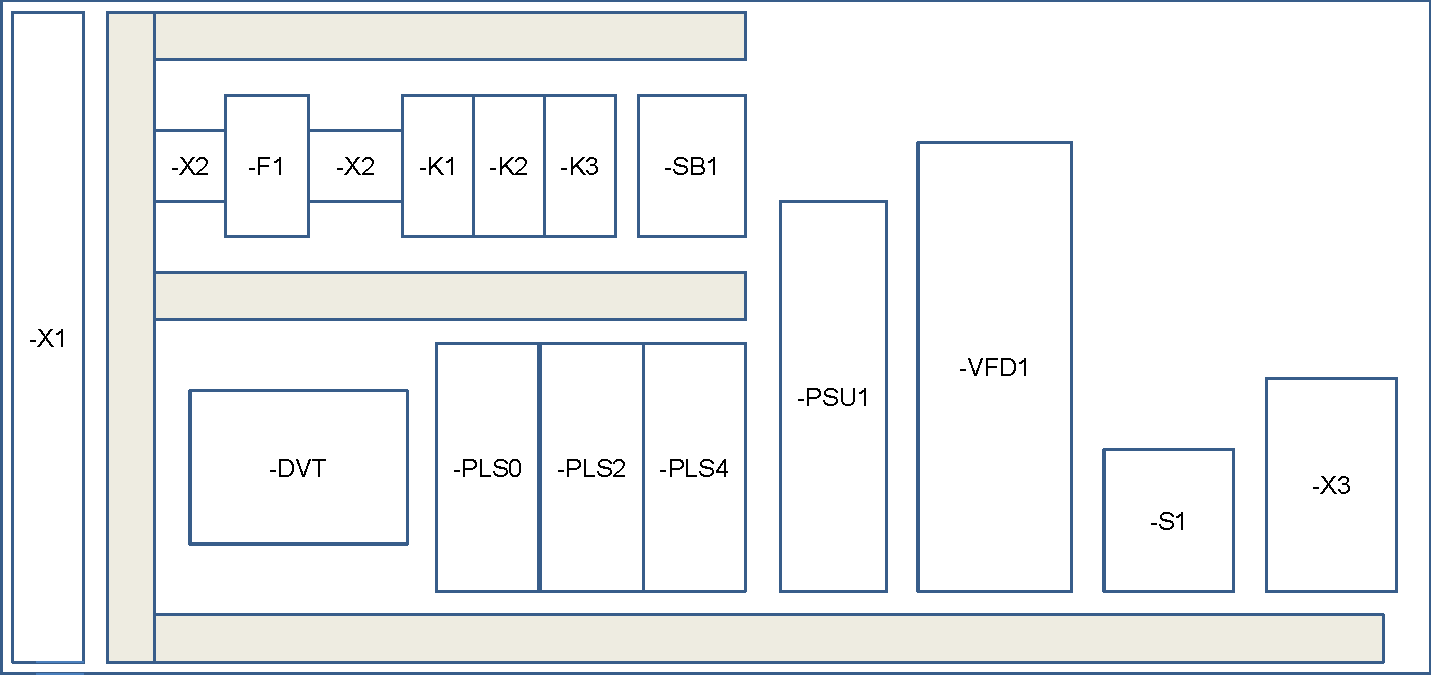
\includegraphics[width=\textwidth]{bilder/arrangementstegning.pdf}
	\caption{Arrangementstegning for koplingsbrettet}
	\label{fig:Arrangementstegning}
\end{figure}







%%%%%%%%%%%%%%%%%%%%%%%%%%%%%%%%%
\subsection{Automatisk sekvens}
\label{subsec:auto}
%%%%%%%%%%%%%%%%%%%%%%%%%%%%%%%%%

Når anlegget settes i automatisk modus, vil systemet kunne jobbe uten menneskelig tilsyn (bokser må settes på båndet manuelt).

%Ved oppstart, og ved kontinuerlig sekvenskjøring må beholder ligge klar i startposisjonen. Posisjonen registreres av FC1, og transportbåndet vil ikke starte ved negativt signal fra sensor. 
Følgende kriterier for start av sekvens må oppfylles (samtidig):

\begin{itemize}
    \item Automatisk modus aktivert i brukergrensesnittet.
    \item Nødstoppbryter S1 ikke aktivert.
    \item Sikkerhetsstrålen ikke brutt -- signal gitt via sikkerhetsmonitor.
    \item Nivåfølerene LZ1 og LZ2 ligger inne.
    \item Materampesensor FC1 aktivert -- beholder i startposisjon.
\end{itemize}
Hvis  alle kriterier er oppfylt, vil transportbåndet starte. Beholderen passerer et lysgitter ved inngangen til en tunnel som leder til visionkameraet. Lysgitteret er beskrevet i underkapittel \ref{sub:sikk}. Visionkameraet fotograferer og tolker en datamatrise, på beholderen, uten å stoppe transportbåndet. Informasjonen som er lagret i datamatrisen, bestemmer  hvordan beholderen skal fylles og behandles videre. Det er satt opp fire alternativer, der de tre første er forskjellige «produkter», og det fjerde er  ikke gjenkjent datamatrise/produkt.

Dersom visionkameraet registerer beholderen som et av de tre produktene, vil sensoren FC3 stoppe båndet når beholderen er under fyllestasjonen. Avhengig av produkt (1, 2 eller 3), vil det fylles forskjellige mengder bulk $A$ og $B$. Disse mengdene bestemmes i brukergrensesnittet. 
 
Ved endt fylling starter transportbåndet. Avhengig av om beholderen skal skyves ut eller ikke, vil en av to sekvenser starte:
 
\begin{enumerate}
     \item Transportbåndet stopper etter en viss tid, for å posisjonere beholderen foran et pneumatisk stempel. %Grunnen til at det brukes en tidsbryter til dette er at det ikke er implementert en sensor for stempelposisjon. 
    Beholderen skyves ut på en siderampe ved at stempelet går ut, fram til giver LZ5 blir aktivert. Deretter går stempelet inn igjen til giver LZ6.
     \item Transportbåndet fortsetter slik at beholderen kjøres av båndet. 
\end{enumerate}

%Hver av disse aksjonene representerer endt sekvens. 
Dersom det innen tre sekunder står klar en ny beholder ved startposisjonen, kjører sekvensen på nytt uten at båndet stoppes. Dersom ingen boks blir detektert,  stoppes båndet. Programmet vil vente på at sensor FC1  detekterer en ny boks, før sekvensen kjøres på nytt. % Dersom ny beholder ikke står i startposisjon innen tre sekund vil sekvensen gå i ventemodus, og det vil kreves et nytt startsignal.



%%%%%%%%%%%%%%%%%%%%%%%%%%%%%%%%%
\subsection{Sikkerhetsmonitor}
\label{sub:sikk}
%%%%%%%%%%%%%%%%%%%%%%%%%%%%%%%%%

Lysgardin og nødstoppbryteren vil alltid stoppe bevegelige deler momentant ved aktivering, uansett om programmet er i automatisk eller manuell modus. For å få til dette er det benyttet en sikkerhetsmonitor. 
PLS-programmet vil gå over  i sikkerhetsmodus, og et passord kreves for opplåsing av denne. Sekvensprogrammet vil ikke starte igjen automatisk -- etter oppheving av sikkerhetsmodus vil programmet gå i manuell modus.



\end{document}